\section{Phương pháp đề xuất}	\label{sec:phuongphapdexuat}
Trong phần này chúng tôi sẽ đặc tả chi tiết bài toán và mô hình hóa phương pháp đề xuất để xây dựng hệ thống phân tích cảm xúc trong văn bản y khoa. Đồng thời chúng tôi cũng trình bày cụ thể các thành phần trong hệ thống và cách sử dụng các thành phần này để giải quyết bài toán.
\subsection{Mô tả bài toán}
Trong luận án này, chúng tôi giải quyết bài toán sau:
Cho câu thuộc 1 bài báo nghiên cứu trong lĩnh vực y khoa, xác định câu đó thuộc 1 trong 3 loại cảm xúc \tichcuc, \tieucuc hoặc \trungtinh. Bài toán gồm 3 yếu tố (Hình \ref{fig:mo-ta-bai-toan}):
\begin{itemize}[noitemsep]
\item[•] Dữ liệu đầu vào: 1 câu trong bài báo nghiên cứu thuộc lĩnh vực y khoa.
\item[•] Kết quả phân tích: \tichcuc, \tieucuc hoặc \trungtinh.
\item[•] Hệ thống phân tích: là phần luận án này xây dựng.
\end{itemize}
\begin{figure}
\centering

\includegraphics[scale=0.35]{../hinh/mo_ta_bai_toan.png}
\caption{Mô tả bài toán} \label{fig:mo-ta-bai-toan}
\end{figure}
Cảm xúc trong luận án này được hiểu như kết quả của 1 phương pháp hay 1 can thiệp, cụ thể:
\begin{itemize}
\item[•] \tichcuc là những câu thể hiện kết quả tốt hơn, cải thiện hơn hoặc kết quả tích cực vượt trội so với tổng thể dù vẫn có tác dụng phụ tiêu cực.\\
\example{1}{\myquote{Patients subjectively reported significantly greater relief from symptoms with Debacterol than with Kenalog-in-Orabase or no treatment.}}
\item[•] \tieucuc là những câu thể hiện kết quả xấu, tệ hơn hoặc thể hiện phương pháp không đem lại hiệu quả.\\
\example{2}{\myquote{There is a suggestion that routine surgical interference may be harmful by increasing the risk of caesarean section, and this agrees with data from other trials.}}
\item[•] \trungtinh là những câu không thể hiện kết quả, không có khẳng định tốt hay xấu; hoặc đồng thời nhiều ý kiến tốt xấu mà không có sự lất át rõ ràng.\\
\example{3}{\myquote{Data extraction and analyses and quality assessment were conducted according to the Cochrane standards.}}
\end{itemize}

\subsection{Kiến trúc tổng quan} \label{subsec:kien-truc-tong-quan}
Chúng tôi đề xuất xây dựng hệ thống phân tích cảm xúc trong báo cáo y khoa theo kiến trúc được mô tả ở Hình \ref{fig:tong-quan-xay-dung-he-thong}. Hệ thống gồm 5 thành phần (\term{modules}) chính: \\

\begin{figure}[H]
\centering
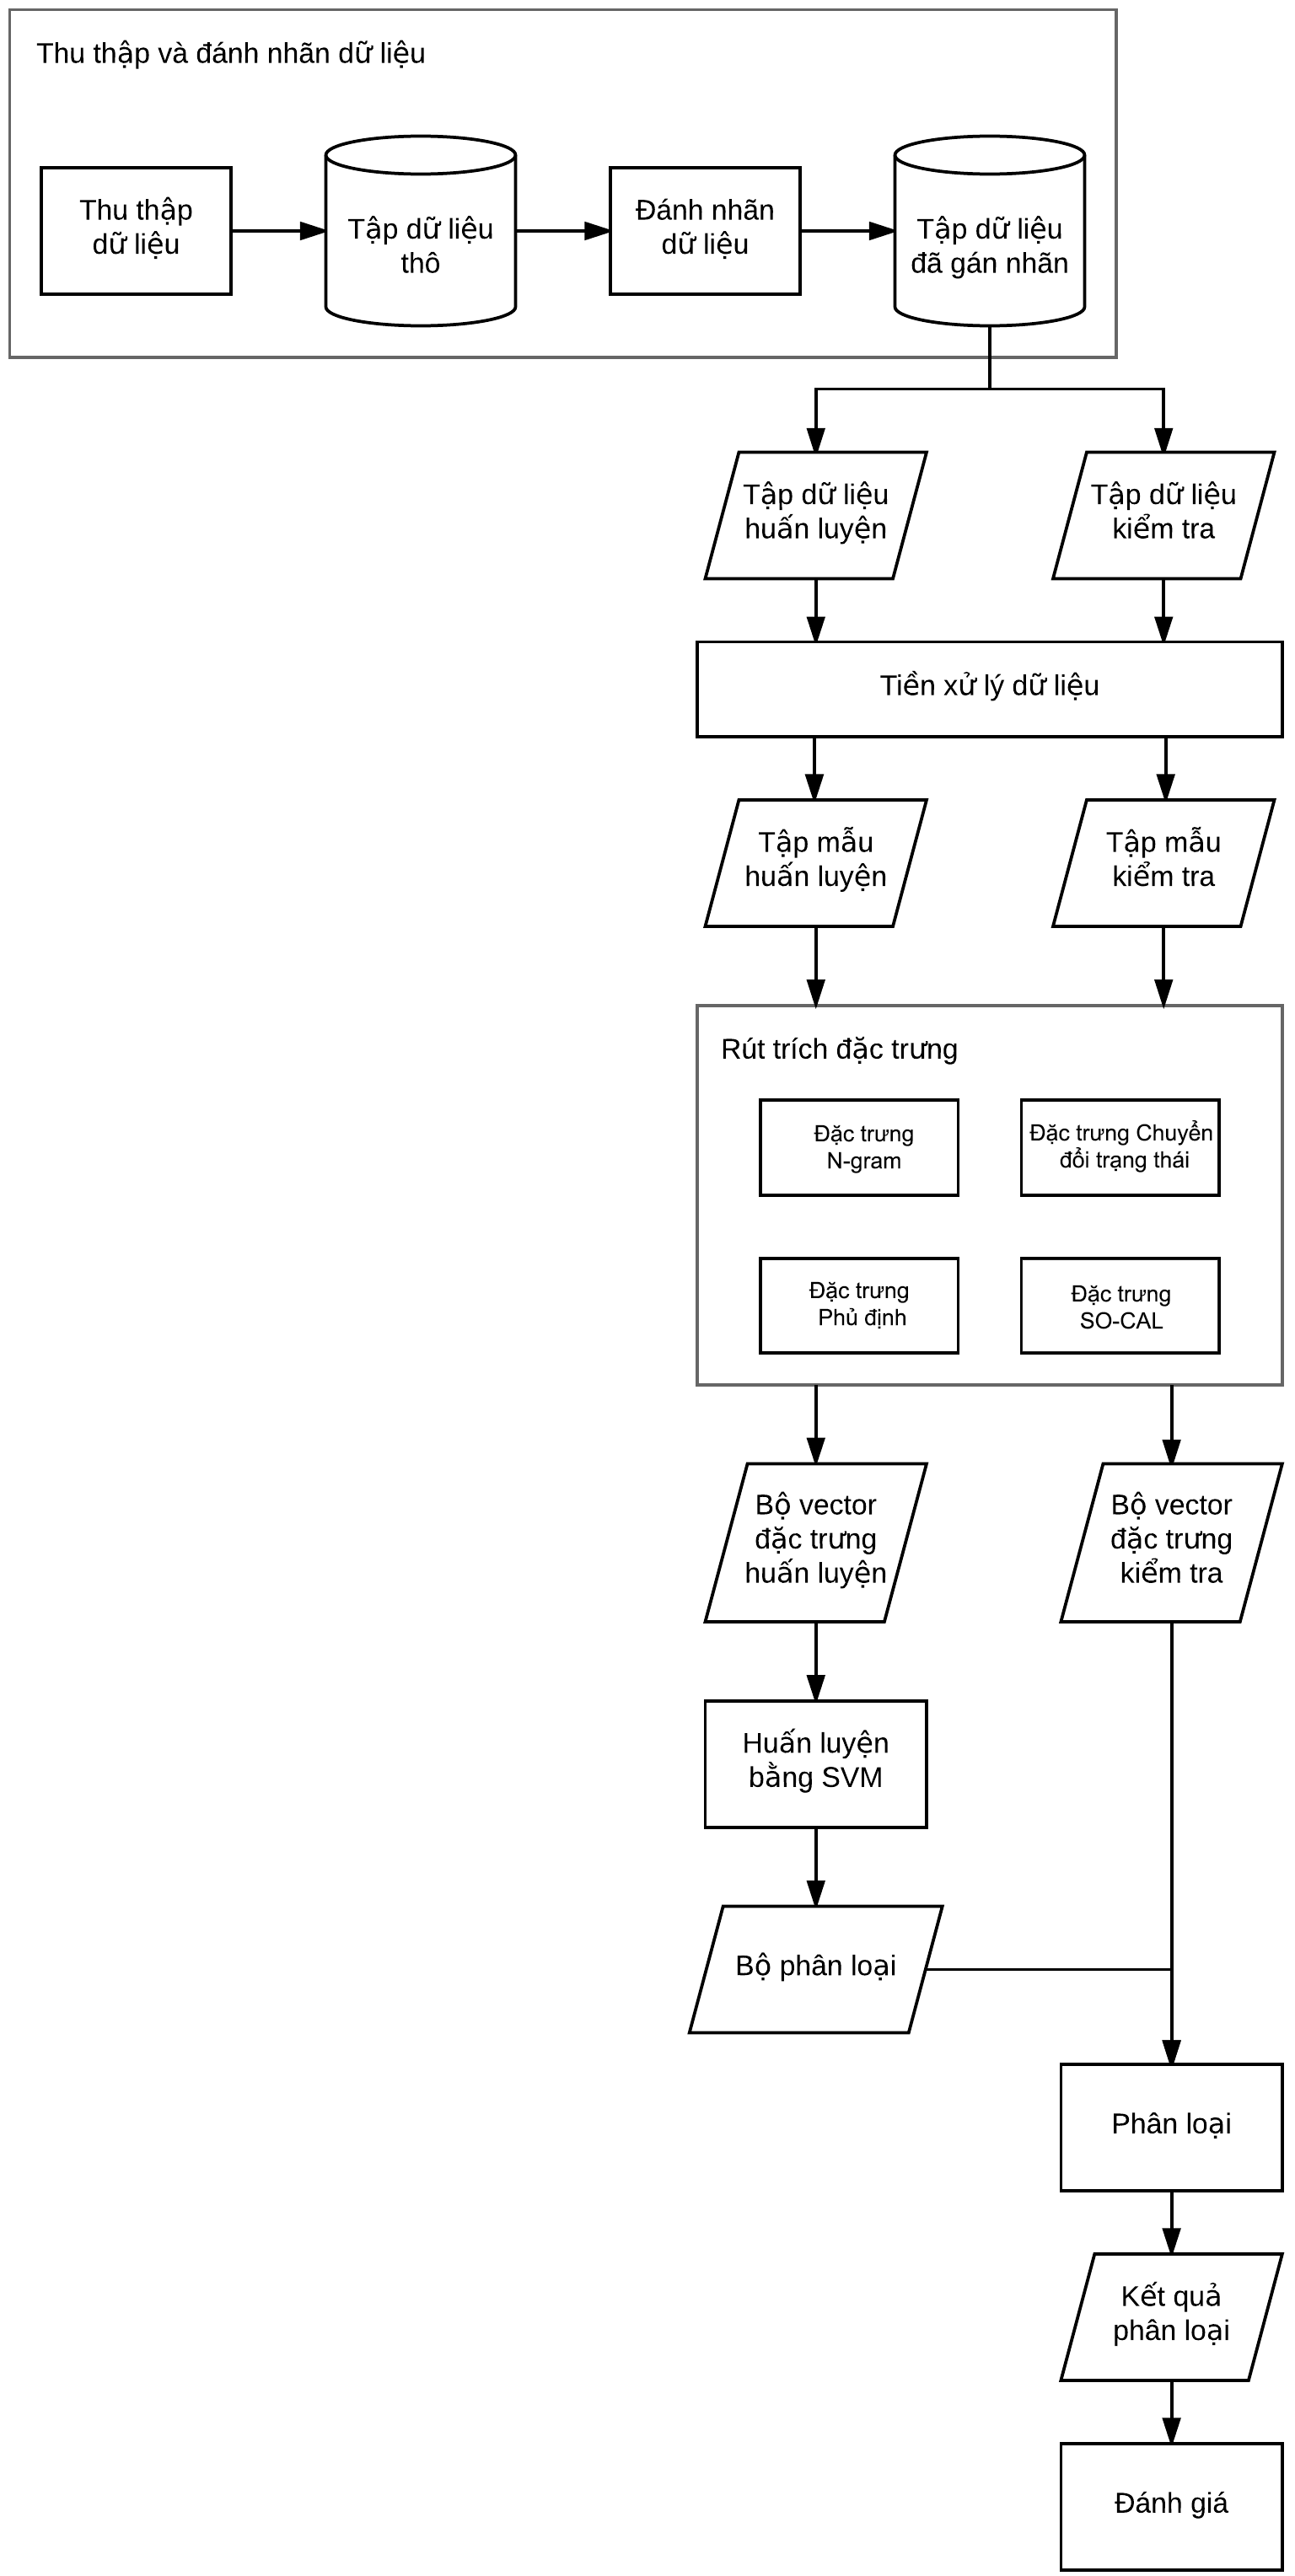
\includegraphics[scale=0.3]{../hinh/Tongquan.png}
\caption{Kiến trúc tổng quan xây dựng hệ thống} \label{fig:tong-quan-xay-dung-he-thong}
\end{figure}

\textbf{Thu thập và đánh nhãn dữ liệu:} Nhóm tiến hành thu thập dữ liệu từ nguồn web, lưu vào hệ cơ sở dữ liệu, sau đó tiến hành đánh nhãn. Chi tiết được trình bày tại Mục \ref{sec:thu-thap-va-danh-gia-du-lieu}.\\

\textbf{Tiền xử lý dữ liệu:} Dữ liệu thu thập được có thể gặp lỗi và có định dạng không đúng, cần được xử lý trước khi trích xuất đặc trưng. \\

Đây là bước xử lý trước khi có thể rút trích đặc trưng. Trong bước này, chúng tôi xử lý dữ liệu theo thứ tự:
\begin{itemize}
\item[•] Chuyển tất cả các ký tự thành chữ thường.
\item[•] Xóa các ký tự đặc biệt, gồm: ?, \%, @, \#, $\wedge$, \$, ., ,,  ;, :, /, ", (, ), +, -, =
\item[•] Thay tất cả số bằng nhãn \term{DIGIT}.
\item[•] Loại bỏ \term{Stop words}: Các từ \term{stop word} là những từ thông thường được sử dụng mà có tính chất phân cực thấp. Một số từ \term{stop word} như: it, I, you, then, \ldots
\item[•] \term{Tokenization}: Sử dụng ký tự khoảng trắng để tách tách câu thành các token
\item[•] \term{Lemmatization:} Trả về dạng đúng của một động từ, dù động từ đó đang ở thì nào. \term{Lemmatization} thực hiện bằng cách loại bỏ đi các biến tố (\term{inflectional}). \\
Ví dụ: ``produced'' -> ``produce''.
\item[•] \term{Stemming} Loại bỏ hầu hết các hậu tố của 1 từ, trả về gốc của một từ dù từ đó được dùng như động từ, tính từ, danh từ hay phó từ.\\
 Ví dụ:  ``produced'' hoặc ``production'' -> ``produc''.
\end{itemize}
\textbf{Rút trích đặc trưng:} Có 4 đặc trưng được sử dụng: N-gram, change phrase, sự phủ định và SO-CAL được trình bày trong các Mục từ \ref{sec:ngram} đến \ref{sec:socal}. \\

\textbf{Huấn luyện:} Thực hiện việc huấn luyện với giải thuật học máy SVM để tạo ra bộ phân loại.\\

\textbf{Phân loại:} Sử dụng bộ phân loại từ khối Huấn luyện, với mỗi dữ liệu đầu vào, bộ phân loại sẽ phân loại câu thuộc 1 trong 3 lớp: \tichcuc,\tieucuc, hoặc \trungtinh\\

\textbf{Đánh giá:} Sử dụng khối phân loại ở trên, áp dụng đầu vào là tập dữ liệu kiểm tra để đánh giá hiệu quả của bộ phân loại.\\

Trong phần còn lại, chúng tôi trình bày các đặc trưng theo cấu trúc 2 phần: Phần Mô tả trình bày ý tưởng, mô tả về đặc trưng, phần Rút trích trình bày cách sử dụng đặc trưng để có thể áp dụng vào hệ thống.


\subsection{Đặc trưng n-gram} \label{sec:ngram}
\subsubsection*{Mô tả}
Theo kết luận của nghiên cứu \cite{chandrakala2012opinion}, n-gram là đặc trưng được sử dụng phổ biến trong bài toán phân tích cảm xúc nói chung. Nhiều nghiên cứu về phân tích cảm xúc trong lĩnh vực y khoa cũng sử dụng đặc trưng này \cite{pang2002thumbs}, \cite{niu2005analysis}, \cite{sarker2011outcome}, \cite{niu2006using}, \cite{pestian2012sentie}, \cite{xia09improving} \\

%Định nghĩa
N-gram là một chuỗi gồm n phần tử liên tiếp nhau. Các phần tử này có thể chữ cái, âm tiết hoặc đoạn văn\ldots Trong nghiên cứu này, các phần tử là các từ đơn trong câu. Đơn vị từ được định nghĩa là chuỗi các chữ cái liên tiếp nhau không chứa ký tự khoảng trắng, các từ phân biệt nhau bởi ký tự khoảng trắng. Đặc trưng n-gram đóng góp lớn trong kết quả của các phân tích, vì vậy đặc trưng này thường được dùng như baseline. Báo cáo  của \cite{pang2002thumbs} phân tích cảm xúc trên các bình luận về phim, đạt độ chính xác 82.9\% với chỉ một đặc trưng n-gram. Đây cũng là kết quả tốt nhất của nghiên cứu này. Nghiên cứu của \cite{niu2005analysis} đạt độ chính xác 77.87\% khi chỉ sử dụng n-gram như \term{baseline}, kết quả tốt nhất tăng 20.58\% so với \term{baseline}.\\

Ví dụ câu: \myquote{Standard practice in pupillary monitoring yields inaccurate data}
\begin{itemize}
\item[•]Với $n=1$, n-gram được gọi là uni-gram. Câu trên sẽ được chuyển thành các n-gram: Standard, practice, in, pupillary, monitoring, yields, inaccurate, data.
\item[•]Với $n=2$, n-gram được gọi là bi-gram. Câu trên sẽ được chuyển thành các n-gram: Standard practice, practice in, in pupillary, pupillary monitoring, monitoring yields, yields inaccurate, inaccurate data.
\item[•]Với $n=3$, n-gram được gọi là tri-gram. Câu trên sẽ được chuyển thành các n-gram: Standard practice in, practice in pupillary, in pupillary monitoring, pupillary monitoring yields, monitoring yields inaccurate, yields inaccurate data.
\item[•]Với $n>3$, tần suất xuất hiện các n-gram thấp, dễ làm mô hình học máy bị học quá khớp (overfitting)
\end{itemize}
	
Việc phối hợp các n-gram là tùy chọn đối với mỗi nghiên cứu, và các kết quả cũng không hoàn toàn đồng nhất. Báo cáo \cite{niu2005analysis} kết luận khi sử dụng bi-gram kết hợp với uni-gram giúp tăng độ chính xác thêm 3.01\%, điều này phù hợp với báo cáo \cite{sarker2011outcome}. Báo cáo \cite{sarker2011outcome} kết luận rằng việc dùng cả uni-gram, bi-gram và tri-gram giúp cải thiện kết quả rõ rệt. Trong khi đó \cite{pang2002thumbs} đạt kết quả cao nhất chỉ với uni-gram. Kết luận của \cite{pang2002thumbs} cho thấy việc sử dụng thêm đặc trưng bi-gram không tác động nhiều đến kết quả. Báo cáo của \cite{smith2012cross} phân tích cảm xúc trong lĩnh vực y khoa lâm sàng, khẳng định đặc trưng uni-gram cho kết quả tốt hơn bi-gram. Tuy nhiên, nghiên cứu không thử nghiệm kết hợp 2 đặc trưng này. Trong báo cáo này, chúng tôi thử nghiệm các cách kết hợp khác nhau của n-gram để tìm ra kết quả tốt nhất.\\

%\subsubsection*{Mở rộng}
TODO Việc áp dụng các kiến thức liên quan đến lĩnh vực đang xem xét giúp tăng độ chính xác khi phân loại. Tác giả Kerstin Denecke trong nghiên cứu \cite{denecke2015sentiment} khẳng định rằng áp dụng kiến thức trong lĩnh vực y khoa là cần thiết để cải thiện hiệu quả phân loại cảm xúc. Trong nghiên cứu này, ý nghĩa cụ thể của các thuật ngữ y khoa không có tác dụng phân loại cảm xúc, chỉ thông tin mô tả của các thuật ngữ này có ý nghĩa.\\

\example{}{\myquote{Elevated troponin level after acute stroke is common and is associated with ECG changes suggestive of myocardial ischemia and increased risk of death}}
Từ \myquote{stroke} xét trong ngữ cảnh y học nghĩa là đột quỵ. Nhưng đối với việc phân loại cảm xúc, chúng tôi chỉ quan tâm tới ý nghĩa khái quát của từ này: \myquote{stroke} mô tả một loại bệnh. Tương tự các từ \myquote{diarrhoea, abdominal pain, nausea} chỉ cần được hiểu như vấn đề về bụng mà không cần hiểu cụ thể như thế nào. Như vậy, các thuật ngữ y khoa thuộc cùng 1 kiểu (triệu chứng, loại bệnh, tên thuốc, ...) đều được xem là một. Từ đó, giảm thiểu khả năng bộ phân loại bị nhiễu hoặc bị học lệch (\term{overfitting}).\\

Một trong những công cụ đã được xây dựng hoàn chỉnh và sử dụng phổ biến trong các bài toán liên quan đến y khoa trên dữ liệu tiếng Anh là UMLS. Đây là một hệ thống tích hợp các thuật ngữ y khoa cùng các mã chuẩn hóa nhằm tạo tiền đề cho việc xây dựng và phát triển các hệ thống thông tin y khoa cũng như các dịch vụ chăm sóc y tế khác. Để hiện thực nhiệm vụ trên, chúng tôi sử dụng công cụ MetaMap kết hợp hệ thống UMLS. UMLS phân các thuật ngữ y học ra làm 136 kiểu \footnote{Chi tiết các kiểu tham khảo tại \texttt{https://metamap.nlm.nih.gov/Docs/SemanticTypes\_2013AA.txt}}. MetaMap là một công cụ cho phép tra cứu tên kiểu của 1 thuật ngữ y học bất kỳ (Hình \ref{fig:metamap}).\\

\begin{figure}[H]
\centering
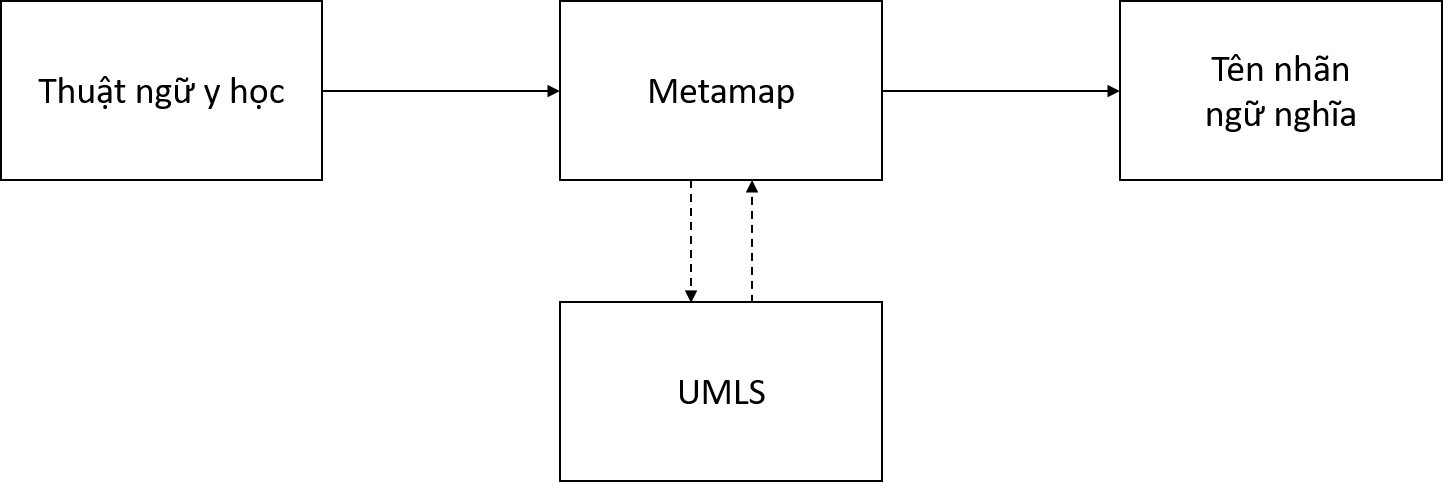
\includegraphics[scale=0.32]{../hinh/metamap.png}
\caption{MetaMap sử dụng nguồn tài nguyên UMLS, giúp tra cứu tên kiểu của 1 thuật ngữ y học}
\label{fig:metamap}
\end{figure}
%Một số ví dụ:\\
\example{1}{
\myquote{Elevated troponin level after acute \underline{stroke} is common and is associated with ECG changes suggestive of myocardial \underline{ischemia} and increased risk of death}\\
$\xrightarrow{MetaMap}$ \\
\myquote{Elevated troponin level after acute \underline{DSYN} is common and is associated with ECG changes suggestive of myocardial \underline{DSYN} and increased risk of death}}
Từ {\myquote{stroke}} và {\myquote{ischemia}} đều thuộc kiểu loại bệnh hoặc triệu chứng, nên được thay bằng nhãn DSYN (Disease or Syndrome)
%\example{2}{
%\myquote{
%In addition, regardless of psychiatric status, \underline{ADHD} placed children at relative risk for educational and vocational disadvantage}\\
%$\xrightarrow{MetaMap}$ \\
%\myquote{In addition, regardless of psychiatric status, \underline{MOBD} placed children at relative risk for educational and vocational disadvantage}\\
%Từ \underline{\myquote{ADHD}} chỉ một dạng rối loạn về thần kinh, nên được thay bằng nhãn MOBD (Mental or Behavioral Dysfunction)\\
%}
\subsubsection*{Rút trích}
Giải thuật trích xuất đặc trưng n-gram trải qua 2 bước, được mô tả như Hình \ref{fig:mo-hinh-ngram}\\
\begin{figure}[H]
\centering
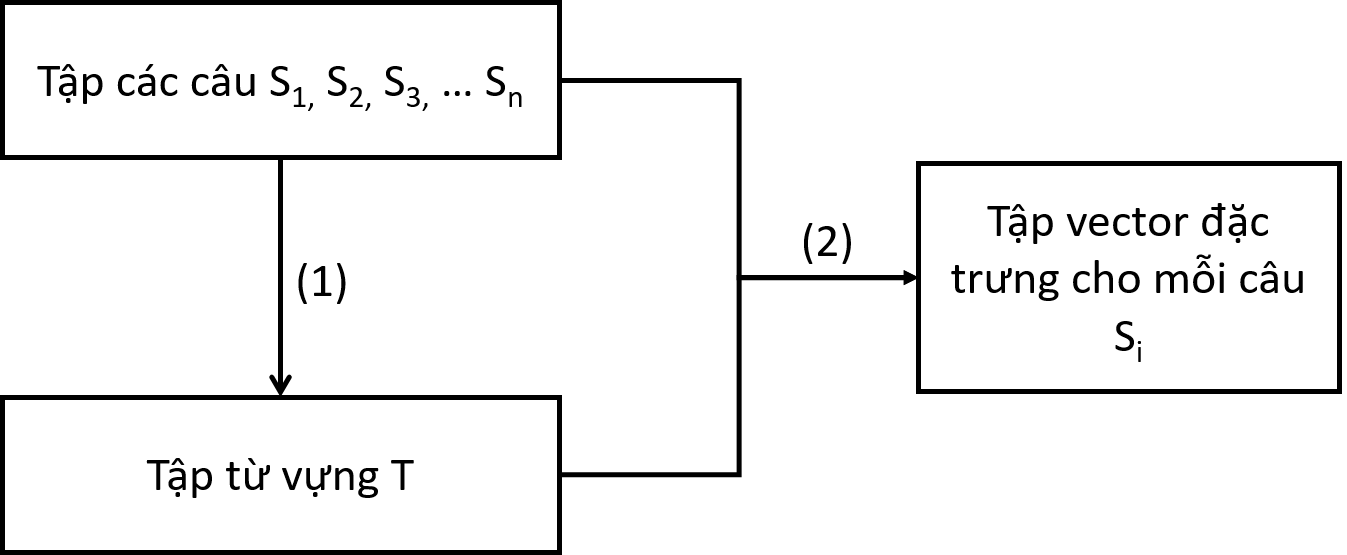
\includegraphics[scale=0.30]{../hinh/mo-hinh-ngram.png}
\caption{Giải thuật trích xuất đặc trưng n-gram} \label{fig:mo-hinh-ngram}
\end{figure}

Ở bước đầu tiên (1), giải thuật nhận vào tập hợp các câu. Mỗi câu sẽ được tách ra thành các n-gram. Tất cả các n-gram từ các câu sẽ được tổng hợp lại thành tập từ vựng T. Tuy nhiên, không phải tất cả các n-gram đều được thêm vào tập từ vựng T. Giải thuật quy định 1 mức ngưỡng $min\_df$ là số câu tối thiểu cùng chứa 1 n-gram thì n-gram đó mới được thêm vào tập T. Nếu $min\_df=1$ thì tập từ vựng T chứa tất cả các n-gram. \\

Nghiên cứu \cite{sarker2011outcome} sử dụng $min\_df = 5$, trong khi nghiên cứu \cite{niu2005analysis} dùng $min\_df=4$. Tuy nhiên cả 2 nghiên cứu trên đều không giải thích về cách chọn các giá trị trên. Trong nghiên cứu này, chúng tôi tiến hành các thí nghiệm để phân tích và chọn ra giá trị $min\_df$ tối ưu nhất.\\

Bước còn lại (2) là \term{vector} hóa câu: ánh xạ 1 câu từ dạng \term{text} sang dạng \term{vector} đại diện cho câu đó. Các n-gram trong tập từ vựng T ở bước (1) được tiến hành sắp xếp. Việc sắp xếp này là tùy ý, nhưng sau khi đã sắp xếp phải giữ nguyên thứ tự. Giả sử $T=\{\text{n-gram}_1, \text{n-gram}_2, \text{n-gram}_3, \ldots, \text{n-gram}_n\}$. Khi đó, mỗi câu $s_i$ sẽ được chuyển thành \term{vector} $v_i$ có n chiều. Có 2 cách hiện thực để xác định giá trị tại chiều thứ $k$ của \term{vector} $v_i$:
\begin{itemize}
\item[•] Giá trị tại chiều thứ $k$ của vector $v_i$ là giá trị nhị phân, bằng 0 nếu câu đó không chứa $\text{n-gram}_k$, bằng 1 nếu câu đó chứa $\text{n-gram}_k$.
\item[•] Giá trị tại chiều thứ $k$ của vector $v_i$ là số nguyên, thể hiện số lần xuất hiện $\text{n-gram}_k$ trong câu đó.
\end{itemize}
Để thuận tiện khi gọi tên trong các thử nghiệm, chúng tôi quy ước đặt tên cách hiện thực thứ nhất là \term{vector nhị phân}, cách hiện thực thứ 2 là \term{vector số nguyên}. \\
\example{3}{
Giả sử sau khi qua bước (1), thu được tập từ vựng T gồm các n-gram: drug, risk, disturbances, associated with, disadvantage, evidence. Khi đó, nếu sử dụng cách vector hóa dùng \term{vector nhị phân}, các câu ở ví dụ 1 và 2 được chuyển thành dạng vector như sau:
}
\begin{tabular}{| c | c | c | c | c | c | c | c |}
\hline
  & \textbf{drug} & \textbf{risk} & \textbf{disturbances} & \textbf{associated with} & \textbf{disadvantage} & \textbf{evidence}
\\ \hline
Ví dụ 1 & 0 & 1 & 0 & 1 & 0 & 0
\\ \hline
Ví dụ 2 & 0 & 1 & 0 & 0 & 1 & 0
\\ \hline
\end{tabular}
Khi đó, $v_1 = (0, 1, 0, 1, 0, 0) $ và $v_2=(0, 1, 0, 0, 1, 0)$
\subsection{Đặc trưng chuyển đổi trạng thái (\term{Change Phrase})}
\subsubsection*{Mô tả}
Đặc trưng change phrase được Niu, Yun et al. định nghĩa trong một nghiên cứu phân tích cảm xúc trên câu \cite{niu2005analysis}. Sau đó được nhóm tác giả Sarker, Abeed, et al. sử dụng lại. Bài toán mà Sarker, Abeed, et al giải quyết cũng tương tự nhưng thay vì phân tích trên câu, nhóm tác giả phân tích trên đoạn. Ngoài việc sử dụng lại, Saker, Abeed,et al. có một số thay đổi và mở rộng đặc trưng này.\\

\textit{Change phrase} là những cụm từ mang ý nghĩa làm thay đổi tình trạng, trạng thái: làm tốt hơn hoặc làm tệ hơn. Tính phân cực trong một câu thường biểu thị qua sự thay đổi \cite{niu2005analysis}, và hay xuất hiện ở những câu so sánh.
\example{}{\myquote{Atypical antipsychotic use is associated with an increased risk for death compared with nonuse among older adults with dementia}}
Câu trên thể hiện tình trạng tệ hơn: Sử dụng \myquote{Atypical antipsychotic} làm tăng nguy cơ chết so với không sử dụng \myquote{Atypical antipsychoti}.
Chúng tôi sử dụng 4 nhóm để mô tả \textit{Change phrase}:
\begin{itemize}
\item[•]Nhóm thể hiện sự thay đổi tình trạng, gồm 2 nhóm:\\
LESS: Có ý nghĩa làm giảm bớt, hạ bớt. Một số từ như: ``reduce'', ``decline'', ``fall'', ``less'', ``little'',\ldots \\
MORE: Có ý nghĩa ngược lại, làm tăng thêm (hoặc duy trì). Một số từ như: ``enhance'', ``higher'', ``exceed'', ``increase'', ``improve'',\ldots
\item[•]Nhóm xác định tính phân cực, gồm 2 nhóm:\\
GOOD: Mang ý nghĩa tích cực. Một số ví dụ như: ``benefit'', ``improvement'', ``advantage'', ``accuracy'', ``great'', \ldots\\
BAD: Mang ý nghĩa tiêu cực. Một số ví dụ như: ''suffer``, ''adverse``, ''hazards``, ''risk``, ''death``,\ldots
\end{itemize}
Danh sách các từ cho mỗi nhóm trên được chúng tôi tập hợp thủ công. Kết hợp 4 nhóm trên, ta có 4 đặc trưng giúp mô tả những thay đổi tích cực hoặc tiêu cực như \refformat{Bảng~\ref{tab:changphrase}}.
\example{}{
\myquote{Atypical antipsychotic use is associated with an increased risk for death compared with nonuse among older adults with dementia}}
Từ \myquote{increased} sẽ được gán nhãn MORE, \myquote{risk} được gán nhãn BAD, sau đó việc phân tích sẽ xác định được đối tượng của từ \myquote{increased} là \myquote{risk}. Từ đó, câu trên được nhận dạng thuộc mẫu MORE-BAD, suy ra nó có xu hướng biểu thị tính phân cực \tieucuc.
\begin{table}[H]
\centering
\caption{Các đặc trưng \textit{Change phrase}}
\label{tab:changphrase}
\begin{tabular}{ | P{0.25\textwidth} | P{0.25\textwidth}| P{0.25\textwidth} | }
\hline
\textbf{Nhóm làm thay đổi tình trạng} & \textbf{Nhóm xác định đối tượng} & \textbf{Phân loại tính phân cực} \\
\hline
LESS & GOOD & \tieucuc \\
\hline
LESS & BAD & \tichcuc \\
\hline
MORE & GOOD	& \tichcuc \\
\hline
MORE & BAD & \tieucuc \\
\hline
\end{tabular}
\end{table}
\subsubsection*{Rút trích}
Rút trích đặc trưng Change phrase phụ thuộc vào 2 yếu tố:
\begin{itemize}
\item[•] Danh sách từ trong mỗi nhóm LESS, MORE, BAD, GOOD
\item[•] Giải thuật nhận biết sự kết hợp của các nhãn trên
\end{itemize}
Với yếu tố thứ nhất, trong nghiên cứu này, chúng tôi sử dụng danh sách từ cho mỗi nhóm tham khảo từ nghiên cứu của nhóm tác giả Sarker, Abeed, et al.\cite{sarker2011outcome}. Nhóm tác giả trên tự tập hợp danh sách các nhóm từ thủ công nhưng không liệt kê trong báo cáo của mình. Nhóm chúng tôi có liên hệ và đã nhận được mã nguồn, từ đó lấy được danh sách các nhóm từ. Danh sách này gồm 371 từ (BAD: 223 từ, GOOD: 82 từ, MORE: 30 từ, LESS:36 từ). Sau đó, chúng tôi mở rộng danh sách bằng cách thu thập thủ công. Danh sách cuối cùng gồm 423 từ (BAD: 238, GOOD: 96, MORE: 42 từ, LESS: 47 từ).\\

Sau khi đã có tập hợp các từ cho mỗi nhóm, chúng tôi xem xét yếu tố thứ 2: hiện thực giải thuật nhận dạng xem 1 câu có thuộc mẫu nào trong 4 mẫu: LESS-GOOD, LESS-BAD, MORE-GOOD, MORE-BAD. Giải thuật nhận dạng câu thuộc mẫu nào được thực hiện qua 2 bước.\\

Ở bước 1, giải thuật nhận dạng những từ mô tả sự thay đổi, bằng cách so trùng các từ trong 2 nhóm LESS và MORE với các từ trong câu. Để có thể so trùng thành công, trước tiên các từ trong 2 nhóm này được xử lý \term{lemmatization} và \term{stemming} như ở mục \ref{subsec:kien-truc-tong-quan}. Sau đó mỗi từ trong câu được so sánh với các từ trong 2 nhóm trên.  Nếu từ $w$ thuộc 1 trong 2 nhóm trên, chuyển sang bước 2, ngược lại tiếp tục với từ tiếp theo.\\

%Nếu từ $w$ thuộc 1 trong 2 nhóm trên, giải thuật thêm \term{tag} ``\_LESS'' hoặc ``\_MORE'' vào cuối các từ thuộc phạm vi từ từ $w$ đến dấu chấm câu (\term{punctuation}) gần nhất (về phía cuối câu). Dấu chấm câu (\term{punctuation}) có thể là dấu chấm (.), dấu phẩy (,), dấu hai chấm (:) hoặc dấu chấm phẩy (;). Ở bước này, đặc trưng Change phrase không thực sự tạo ra một đặc trưng mới, nó chỉ làm thay đổi các n-gram: từ risk thành risk\_MORE, từ đó thay đổi tập từ vựng T của đặc trưng n-gram . Bằng cách này, thông qua đặc trưng n-gram, Change phrase không chỉ nhận biết được trong câu có sự mô tả về thay đổi, mà còn biết được phạm vi ảnh hưởng của sự thay đổi đó.\\
%\example{}{\myquote{Atypical antipsychotic use is associated with an increased risk for death compared with nonuse among older adults with dementia}}
%Giải thuật sẽ đánh dấu \term{tag} \_MORE từ từ increased đến hến câu:  \myquote{Atypical antipsychotic use is associated with an increased risk\_MORE for\_MORE death\_MORE compared\_MORE with\_MORE nonuse\_MORE among\_MORE older\_MORE adults\_MORE with\_MORE dementia\_MORE}\\

Bước 2 nhận diện xem câu có thuộc mẫu nào trong 4 mẫu: LESS-GOOD, LESS-BAD, MORE-GOOD, MORE-BAD hay không. Nếu trong câu có 1 từ thuộc nhóm MORE, giải thuật sẽ xác định trong phạm vi từ từ đó đến hết câu, nếu có từ nào thuộc nhóm GOOD, câu đó thuộc mẫu MORE-GOOD. Tương tự như vậy đối với 3 mẫu còn lại.\\

Cuối cùng, mỗi câu được chuyển thành 1 vector 4 chiều. Giá trị tại chiều thứ $i$ bằng 1 nếu câu thuộc mẫu thứ $i$, ngược lại bằng 0. Thứ tự các mẫu được sắp xếp như sau: MORE-GOOD, MORE-BAD, LESS-GOOD, LESS-BAD

\subsection{Đặc trưng phủ định} \label{sec:su-phu-dinh}
\subsubsection*{Mô tả}
Bài toán phân tích phủ định bao gồm hai nhiệm vụ chính là (1) xác định yếu tố phủ định cùng với phạm vi phủ định trong câu và (2) phân tích ảnh hưởng cũng như hiệu quả của yếu tố phủ định lên ý nghĩa phân loại tính phân cực của cả câu. Để giải quyết bài toán này chúng tôi đã tìm hiểu và hiện thực lại giải thuật phân tích phủ định NegEx\cite{Tanushi2013} (chi tiết hiện thực được mô tả cụ thể ở chương \ref{sec:hienthuchethong}).\\
%\footnote{https://code.google.com/archive/p/negex/}. \\

Giải thuật NegEx dùng để xác định sự tồn tại của phủ định trong câu và xác định xem một cụm từ bất kỳ trong câu có chịu ảnh hưởng của yếu tố phủ định hay không. Giải thuật nhận dữ liệu đầu vào là câu văn được nghi ngờ có sự phủ định và một cụm từ thuộc câu văn đó mà cần xác định xem có bị phủ định hay không. Sau quá trình xử lý, giải thuật đưa ra câu trả lời gồm: câu văn có tồn tại sự phủ định không, xác định từ phủ định trong câu và cụm từ được hỏi có bị phủ định hay không.\\ 

Trong quá trình xử lý, NegEx dùng danh sách thuật ngữ phủ định và danh sách thuật ngữ kết thúc để giải quyết bài toán. Bên cạnh đó, giải thuật xây dựng hai biểu thức chính quy \myquote{RE} (\term{regular expressions}) để xác định phạm vi phủ định trong câu. Biểu thức \myquote{RE1} bao gồm tất cả các từ (từ đơn hoặc cụm từ) đứng sau thuật ngữ phủ định và sẽ kết thúc bởi một thuật ngữ kết thúc hoặc dấu kết thúc câu hoặc một thuật ngữ phủ định khác. Biểu thức \myquote{RE2} chỉ xác định khoảng 5 từ (từ đơn hoặc cụm từ), ưu tiên lĩnh vực y khoa đứng trước thuật ngữ phủ định đang xét. \\

Áp dụng vào bài toán, với mỗi câu trong dữ liệu đầu vào, giải thuật NegEx lặp lại theo các bước sau:

\begin{enumerate}
\item Xác định tất cả các từ phủ định có trong câu dựa trên danh sách thuật ngữ phủ định, ký hiệu là tập \textit{A}.
\item Tìm từ phủ định đầu tiên trong câu, kí hiệu là \textit{Neg1}.
\item Nếu \textit{Neg1} là từ phủ định giả, bỏ qua và thực hiện bước 6.
\item Nếu \textit{Neg1} là từ phủ định tiền điều kiện: dùng biểu thức chính quy \myquote{RE1} xác định vùng phủ định của \textit{Neg1}.
\item Nếu \textit{Neg1} là từ phủ định tiền điều kiện: dùng biểu thức chính quy \myquote{RE2} xác định vùng phủ định của \textit{Neg1}.
\item Tìm từ phủ định kế tiếp (cho đến khi hết các từ trong tập \textit{A}), gán cho \textit{Neg1} và lặp lại bước 3.
\end{enumerate}

Một số ví dụ khi chạy giải thuật NegEx:

\example{8}{\myquote{Patients subjectively reported significantly greater relief from symptoms with Debacterol than with Kenalog-in-Orabase or ([no] treatment).}\\Từ phủ định tìm được: \myquote{no} là thuật ngữ phủ định tiền điều kiện, phạm vi phủ định được xác định, từ bị phủ định là \myquote{treatment}.}

\example{9}{\myquote{The patient is (tumor [free]).}\\Từ phủ định tìm được: \myquote{free} là thuật ngữ phủ định hậu điều kiện, phạm vi phủ định được xác định, từ bị phủ định là \myquote{tumor}.}
\subsubsection*{Rút trích}
Sau khi đã xác định được từ phủ định và từ chịu ảnh hưởng phủ định trong câu, chúng tôi thực hiện rút trích đặc trưng phủ định theo 3 cách sau để áp dụng vào hệ thống:\\

%The authors drew interesting results such as that adding negation as an explicit feature with uni- grams and using POS tags are not useful for polarity classification. They also reported that the most effective methodwas usingNBwith bigrams as features,which managed to achieve an accuracy of 82.7\%.

Cách thứ nhất tham khảo từ nghiên cứu \cite{niu2005analysis}. Trong nghiên cứu đó, nhóm tác giả \\TODO <thêm tên> chỉ xem xét 1 từ phủ định ``no''. Đây có thể là sự thiếu sót của nhóm tác giả, vì kết quả trong báo cáo \cite{niu2005analysis} cho thấy yếu tố phủ định được thêm vào hầu như không giúp cải thiện độ chính xác. Tiếp theo, nhóm tác giả trên sử dụng công cụ Apple Pie parser để trích xuất các cụm từ, cụm từ nào có chứa từ ``no'' sẽ được gắn thêm hậu tố ``\_NO''. Với cách này, yếu tố phủ định không thực sự là 1 đặc trưng mà chỉ ảnh hưởng đến hệ thống thông qua đặc trưng n-gram. Chúng tôi thử nghiệm cách này nhưng thay vì chỉ quan tâm đến từ ``no'', chúng tôi xem xét đến tất cả các từ được xem là từ phủ định theo giải thuật được mô tả ở phần trước. Sau đó, các từ được xem là chịu ảnh hưởng phủ định được thêm hậu tố ``\_NEG''.

\example{}{
Câu: \myquote{
Patients subjectively reported significantly greater relief from symptoms with Debacterol than with Kenalog-in-Orabase or ([no] treatment)}\\
sẽ được chuyển thành: \\
\myquote{
Patients subjectively reported significantly greater relief from symptoms with Debacterol than with Kenalog-in-Orabase or no treatment\_NEG}
}

Cách thứ 2 chúng tôi thử nghiệm có tác dụng tương tự cách trên: không thực sự là 1 đặc trưng mà chỉ ảnh hưởng đến đặc trưng n-gram. Nhưng thay vì làm thay đổi từ bị ảnh hưởng phủ định, cách hiện thực này thay  đổi từ phủ định: thay tất cả các từ phủ định bằng nhãn đại diện ``NEGATION''\\

\example{}{
Câu: \myquote{
Patients subjectively reported significantly greater relief from symptoms with Debacterol than with Kenalog-in-Orabase or ([no] treatment)}\\
sẽ được chuyển thành: \\
\myquote{
Patients subjectively reported significantly greater relief from symptoms with Debacterol than with Kenalog-in-Orabase or NEGATION treatment}
}

Cách còn lại cũng chỉ quan tâm đến từ phủ định, nhưng khác 2 cách trên: cách hiện thực này tạo ra 1 vector đại diện chứ không làm ảnh hưởng đến đặc trưng n-gram. Mỗi câu sẽ được ánh xạ thành 1 số nhị phân: 0 nếu câu đó không chứa yếu tố phủ định nào, 1 nếu ngược lại.\\

Ngoài ra, chúng tôi cũng tiến hành thử nghiệm kết hợp các cách hiện thực trên để tìm ra cách rút trích hiệu quả nhất.
\subsection{Đặc trưng mở rộng SO-CAL} \label{sec:socal}
\subsubsection*{Mô tả}
Trong nghiên cứu này, chúng tôi sử dụng đặc trưng SO-CAL dựa trên bài báo \cite{taboada2011lexicon}, tên của đặc trưng xuất phát từ tên hệ thống mà bài báo trên đã xây dựng. Theo ý nhóm tác giả \cite{taboada2011lexicon}, SO-CAL là chữ viết tắt của Semantic Orientation CALculator. Đây là một phương pháp phân tích cảm xúc dựa trên từ vựng.\\

Phân tích cảm xúc dựa trên từ vựng là một phương pháp khác, tránh được bất lợi của phương pháp học máy là không cần qua quá trình huấn luyện. Tuy nhiên đa số các nghiên cứu này đều phân tích cảm xúc trên văn bản thông thường, không tập trung vào 1 lĩnh vực cụ thể nào \cite{taboada2011lexicon,Zhang2011,ohana2009sentiment,Giachanou2016}. \\

Phương pháp này ngầm định 2 giả thiết sau đã được thỏa mãn:
\begin{itemize}
\item[•] Bản thân mỗi từ có sẳn tính phân cực mà không bị phụ thuộc vào ngữ cảnh. Điều này có nghĩa là mỗi từ luôn chỉ có 1 xu hướng phân cực (tốt, xấu hoặc tích cực, tiêu cực) trong mọi câu mà từ đó xuất hiện.
\item[•] Tính phân cực của mỗi từ được đề cập ở trên có thể được biểu diễn bởi 1 số thực
\end{itemize}
Dựa trên 2 giả thiết trên, tính phân cực của một câu phụ thuộc vào số thực biểu diễn tính phân cực của các từ trong câu đó, và cũng được biểu diễn bởi 1 số thực. Sự phụ thuộc giữa tính phân cực của các từ và tính phân cực của cả câu là tùy thuộc vào các nghiên cứu, có thể mô hình hóa như công thức sau:
\begin{equation}
Polarity_{sentence}=f(Polarity_{words-in-sentence})
\end{equation}
\subsubsection*{Rút trích}
Rút trích đặc trưng SO-CAl chính là giải thuật tính điểm số cho mỗi câu phụ thuộc vào điểm số của mỗi từ trong câu. Sau đây, chúng tôi trình bày các vấn đề chính khi tính điểm cho từ
\paragraph*{Từ điển}
Đây là công cụ giúp tra cứu điểm số của mỗi từ. Các từ điển hiện nay thuộc 2 loại: xây dựng thủ công hoặc xây dựng bán tự động. Từ điển xây dựng thủ công điển hình được sử dụng nhiều trong các nghiên cứu là bộ từ điển General Inquirer. Lợi thế của loại tự điển này là được con người đánh điểm số, vì vậy giảm thiếu sai sót. Các nghiên cứu có thể dựa trên bộ từ điển này để tự mở rộng thành bộ từ điển của mình. Tuy nhiên, bất lợi của loại này là kích thước thường nhỏ. Bộ từ điển thuộc loại thứ 2 được sử dụng phổ biến là WordNet. Từ điển thuộc loại bán tự động được xây dựng bằng cách sử dụng một tập từ hạt giống có tính phân cực cao. Các từ này có thể được tập hợp thủ công hoặc được lấy từ từ điển General Inquirer. Từ đó, điểm của các từ khác được sinh ra dựa trên tần số xuất hiện của chúng so với các từ hạt giống. Lợi thế của loại từ điển này là kích thước lớn, tạo độ bao phủ cao, từ đó nhiều từ được gán điểm số hơn. Tuy nhiên độ chính xác của loại từ điển này không cao, và kích thước lớn thường đi kèm với nhiễu. \\

Nghiên cứu \cite{taboada2011lexicon} vì thế chọn phương án xây dựng một bộ từ điển thủ công dựa trên một số nguồn text như các bình luận về phim, sách, máy tính, khách sạn,... và các từ thuộc nhóm tích cực, tiêu cực từ từ điển General Inquirer. Điểm số mỗi từ trong từ điển được xây dựng có giá trị từ -5 đến 5 với ý nghĩa: Giá trị càng nhỏ thể hiện tính phân cực về phía tiêu cực càng nhiều, và ngược lại. 
\begin{table}[H]
\begin{tabular}{l l}
\hline
\textbf{Từ} & \textbf{Giá trị} 
\\ \hline
monstrosity & -5
\\ 
hate (noun and verb) & -4
\\ 
disgust & -3
\\ 
sham & -3
\\ 
fabricate & -2
\\ 
delay (noun and verb) & -1
\\
determination & 1
\\
determination & 1
\\ 
inspire & 2
\\ 
inspiration & 2
\\ 
endear & 3
\\ 
relish (verb) & 4
\\ 
masterpiece & 5
\\ \hline
\end{tabular}
\end{table}
\paragraph*{Từ loại}
Hầu hết các nghiên cứu ban đầu về phân tích cảm xúc dựa trên từ vừng đều chỉ tập trung vào tính từ. Điểm số của cả văn bản chỉ phụ thuộc vào điểm số của tính từ trong câu và những từ liên quan. 
Xét 2 ví dụ sau: 
\begin{itemize}
\item[•] \myquote{The young man strolled+ purposefully+ through his neighborhood+}
\item[•] \myquote{The teenaged male strutted- cockily- through his turf-}
\end{itemize}
Các dấu + ở câu thứ nhất thể hiện xu hướng bổ sung tích tích cực vào độ phân cực của cả câu, trong khi dấu - ở ví dụ thứ 2 ngược lại. Từ đó cho thấy, ngoài tính từ, các từ loại động từ, danh từ và phó từ cũng có tác động đến điểm số phân cực của cả câu. Các nghiên cứu sau này đã mở rộng hơn, ngoài tính từ, các từ loại động từ, danh từ và phó từ cũng được xem xét tới. \\

Điều này không những giúp đánh giá tốt hơn trong trường hợp ví dụ trên, ngoài ra còn giúp giải quyết một số trường hợp đặc biệt khi một từ có thể thuộc nhiều loại từ loại. Ví dụ: từ \myquote{novel} nếu xét theo từ loại danh từ thì chỉ mang ý nghĩa trung tính, nếu xét theo từ loại tính từ lại có ý nghĩa tích cực. Từ \myquote{plot} mang ý nghĩa tiêu cực nếu là động từ, nhưng mang tính nghĩa trung tính nếu xem là danh từ. Trong nghiên cứu \cite{taboada2011lexicon}, bộ từ điển được xây dựng gồm 2252 tính từ, 1142 danh từ, 903 động từ, and 745 phó từ. \\

Tất cả các động từ và danh từ trong từ điển đều được xử lý \term{lemmatized}, vì vậy các động từ ở các dạng thể hiện khác nhau đều cùng 1 điểm số. Các động từ, danh từ và tính từ đều được đánh điểm thủ công, riêng phó từ được đánh điểm tự động dựa trên tính từ. Phó từ được bỏ đuôi ``-ly'', sau đó so trùng với các tính từ. Ví dụ: từ \myquote{purposefully} sẽ được gán điểm số của tính từ \myquote{purposefull}. Tuy nhiên, một số ngoại lệ như các phó từ \myquote{fast} được xử lý thủ công. 
\paragraph*{Tính tăng cường (intensification)}
Một từ có tính tăng cường được hiểu là các từ bản thân nó không có điểm số thể hiện tính phân cực, nhưng có khả năng tác động lên 1 từ khác, làm tăng lên hoặc hạ thấp tính phân cực của từ đó. Từ đó làm thay đổi điểm số thể hiện tính phân cực của cả cụm từ. Một số từ có tính tăng cường như: \myquote{slightly}, \myquote{very}, \myquote{most}, \myquote{the most}. Một giải thuật đơn giản có thể được sử dụng trong trường hợp này như sau:
Khi gặp một từ có tác động làm tăng tính phân cực (\myquote{very}), điểm của từ bị tác động được cộng thêm 1 hằng số. 
Cụm từ \myquote{very good} được tính điểm bằng công thức: $Polarity(\text{\myquote{very good}}) = P(\text{\myquote{good}}) + 1$.
Tương tự với trường hợp còn lại. \\

Tuy nhiên cách hiện thực này không thể hiện đúng bản chất của tác động tăng cường. Bởi vì cùng một từ \myquote{very} có thể có tác động mạnh yếu khác nhau tùy thuộc vào từ bị tác động. Nói cách khác, sự tác động này nên phụ thuộc vào cả 2 thành phần: 
\begin{itemize}
\item[•] Tính chất tăng cường của từ tác động. Tính chất này có thể được thể hiện bằng tỉ lệ phần trăm (\%) như Bảng \ref{table:intensive}.
\item[•] Tính phân cực của từ bị tác động
\end{itemize}
Nghiên cứu \cite{taboada2011lexicon} sử dụng công thức (\ref{equa:intensive}) để tính điểm số trong trường hợp này:
\begin{equation}
\label{equa:intensive}
Polarity (\text{cụm từ}) = Polarity(\text{từ bị tác động}) * (100\% - \text{tỉ lệ tác động})
\end{equation}
\begin{table}[H]
\centering
\caption{Tỉ lệ tác động của một số từ} \label{table:intensive}
\begin{tabular}{l l}
\hline
\textbf{Từ} & \textbf{Tỉ lệ tác động} 
\\ \hline
slightly & -50\%
\\ 
somewhat & -30\%
\\ 
pretty & -10\%
\\ 
really & +15\%
\\ 
very & +25\%
\\ 
extraordinarily & +50\%
\\
(the) most & +100\%
\\ \hline
\end{tabular}
\end{table}
\example{}{
\myquote{good} có điểm số là 3.0, từ đó \myquote{very good} có điểm số là: 3.0 * (100\% + 25\%) =  3.75}
Trong trường hợp có hơn 1 từ có tính tăng cường, điểm số được tính tương tự theo cách đệ quy. \\
\example{}{\myquote{really very good}: (3 * [100\% + 25\%]) * (100\% + 15\%) = 4.3}

Trong trường hợp một tính từ bổ sung nghĩa cho một danh từ theo sau nó, tính từ đó được coi như là một từ có tính tăng cường. Vì vậy, bản thân tính từ đó không có điểm số, và chỉ làm thay đổi điểm số của danh từ theo sau. \\

\example{}{
\myquote{This is a total failure}\\
Tính từ \myquote{total} được xem là từ có tính tăng cường, nên thay vì sử dụng điểm số, \myquote{total} ảnh hưởng đến điểm số của \myquote{failure}: $-3.0 * (100\% + 50\%) = -4.5$
}
\paragraph*{Xử lý phủ định}
Sự xuất hiện từ phủ định có thể làm đảo chiều tính phân cực cho cả câu. Tuy nhiên, một từ phân cực về phía tiêu cực mạnh (điểm số rất thấp), không có nghĩa rằng sẽ phân cực về phía tích cực mạnh (điểm số rất cao). Nghiên cứu \cite{taboada2011lexicon} sử dụng chiến lược \term{shift negation}. Thay vì chỉ đơn thuần đổi dấu điểm số, \term{shift negation} chỉ cộng/trừ 1 lượng cố định (trong nghiên cứu này là 4) vào điểm số của từ bị phủ định.\\

\example{}{
\myquote{This CD is not horrid}\\
Điểm số của \myquote{horrid} là -5, khi đó, \myquote{not horrid} có điểm số là: -5 + 4 = -1
}

\paragraph*{Tính điểm số cho câu}
Sau khi đã tính điểm cho các từ, SO-CAL tính điểm cho câu dựa trên nguyên tắc: Lấy trung bình cộng điểm số những từ có điểm số khác 0. Trường hợp tất cả các từ có điểm số bằng 0 thì điểm số của câu cũng bằng 0
